\documentclass[a4paper,10pt]{article}

%\usepackage{natbib}
\usepackage{amsthm}
\usepackage{amsfonts}
\usepackage{amssymb}
\usepackage{amsmath}
\usepackage{latexsym}
\usepackage{graphicx}
\usepackage{blindtext}

\usepackage{doc}

\newtheorem*{theorem}{Theorem}
\theoremstyle{definition}
\newtheorem*{definition}{Definition}

\hoffset -1in \topmargin 0mm \voffset 0mm \headheight 0mm
\headsep0mm
\oddsidemargin  20mm     %   Left margin on odd-numbered pages.
\evensidemargin 20mm     %   Left margin on even-numbered pages.
\textwidth   170mm       %   Width of text line.
\textheight  252mm

\makeatletter
\renewcommand\@openbib@code{%
     \advance\leftmargin  \z@ %\bibindent
      \itemindent \z@
     % Move bibitems close together
     \parsep -0.8ex
     }
\makeatother

\makeatletter
\renewcommand\section{\@startsection {section}{1}{\z@}%
                                   {-3.5ex \@plus -1ex \@minus -.2ex}%
                                   {1.5ex \@plus.2ex}%
                                   {\large\bfseries}}
\makeatother

\makeatletter
\renewcommand\subsection{\@startsection {subsection}{1}{\z@}%
                                   {-3.5ex \@plus -1ex \@minus -.2ex}%
                                   {1.5ex \@plus.2ex}%
                                   {\normalsize\bfseries}}
\makeatother

\makeatletter
	\setlength{\abovecaptionskip}{3pt}   % 0.25cm 
	\setlength{\belowcaptionskip}{3pt}   % 0.25cm 
\makeatother

\begin{document}
\pagestyle{empty}

\begin{center}
{\bf \Large TITLE OF SEMINAR PAPER}
\end{center}

\smallskip
\begin{center}
{\large Author Name (Name Surname)}
\end{center}

\smallskip
\begin{center}
Faculty of Mechanical Engineering, Brno University of Technology\\
Institute of Automation and Computer Science\\
Technicka 2896/2, Brno 616 69, Czech Republic\\
Name.Surname@vutbr.cz\\
\end{center}

\bigskip
\noindent Abstract: \textit{This is a sample of the format of your
full paper. For text in abstract and keywords, use Italics, 10pt. Leave one blank line after the Abstract.}

\vspace*{10pt} \noindent Keywords: \textit{Write your keywords (6--10 words).
Leave a double blank line after your keywords.}

\bigskip
\section{Introduction}
\label{sec:1}
\blindtext

\section{Problem Formulation (Equations)}
\label{sec:2}
Mathematical equations must be centered and numbered as follows:~\eqref{eq:01},~\eqref{eq:02},$\ldots$, (99).
\begin{equation}z^{EO}=\min\limits_{e,\,g(\xi)}\mathbb{E}(F(\xi,e,g(\xi))),
\label{eq:01}
\end{equation}
\begin{equation} a_{min}\leq a\leq a_{max}.
\label{eq:02}
\end{equation}

\subsection{Subsection}
\label{subsec:1}
When including a subsection you must use, for its heading, small
letters, 10pt, left justified bold as here.
Use the standard \verb|equation| environment to typeset your equations, however, for multiline equations we recommend to use the \verb|eqnarray| environment (\LaTeX{} users).

\begin{definition}
Let $H$ be a subgroup of a group~$G$.  A \emph{left coset}
of $H$ in $G$ is a subset of $G$ that is of the form $xH$,
where $x \in G$ and $xH = \{ xh : h \in H \}$.
Similarly a \emph{right coset} of $H$ in $G$ is a subset
of $G$ that is of the form $Hx$, where
$Hx = \{ hx : h \in H \}$
\end{definition}

\begin{theorem}
This is a theorem content. Theorem text goes here. 
\end{theorem}

\begin{proof}
Let $z$ be some element of $xH \cap yH$.  Then $z = xa$
for some $a \in H$, and $z = yb$ for some $b \in H$.
If $h$ is any element of $H$ then $ah \in H$ and
$a^{-1}h \in H$, since $H$ is a subgroup of $G$.
However, $zh = x(ah)$ and $xh = z(a^{-1}h)$ for all $h \in H$.
Therefore $zH \subset xH$ and $xH \subset zH$, and thus
$xH = zH$.  Similarly $yH = zH$, and thus $xH = yH$,
as required.
\end{proof}

\section{Problem Solution}
Figures\footnote{If you copy text passages, figures, or tables from other works, you must obtain \textit{permission} from the copyright holder (usually the original publisher or author). Please enclose the signed permission with the manuscript.} and tables should be numbered as follows: Fig.~1,
Fig.~2,\,\dots{} etc. (see Fig.~\ref{fig:1}), Table 1, Table 2,\,\dots{} etc. (see Table~\ref{tab:1}). Figure caption must be placed below the figure and table caption must be placed above the table. Some reference \cite{SICILIANO_rhandbook}.

%
% For figures use (also *.eps, *.tiff)
%
\begin{figure}[h]
\begin{center}
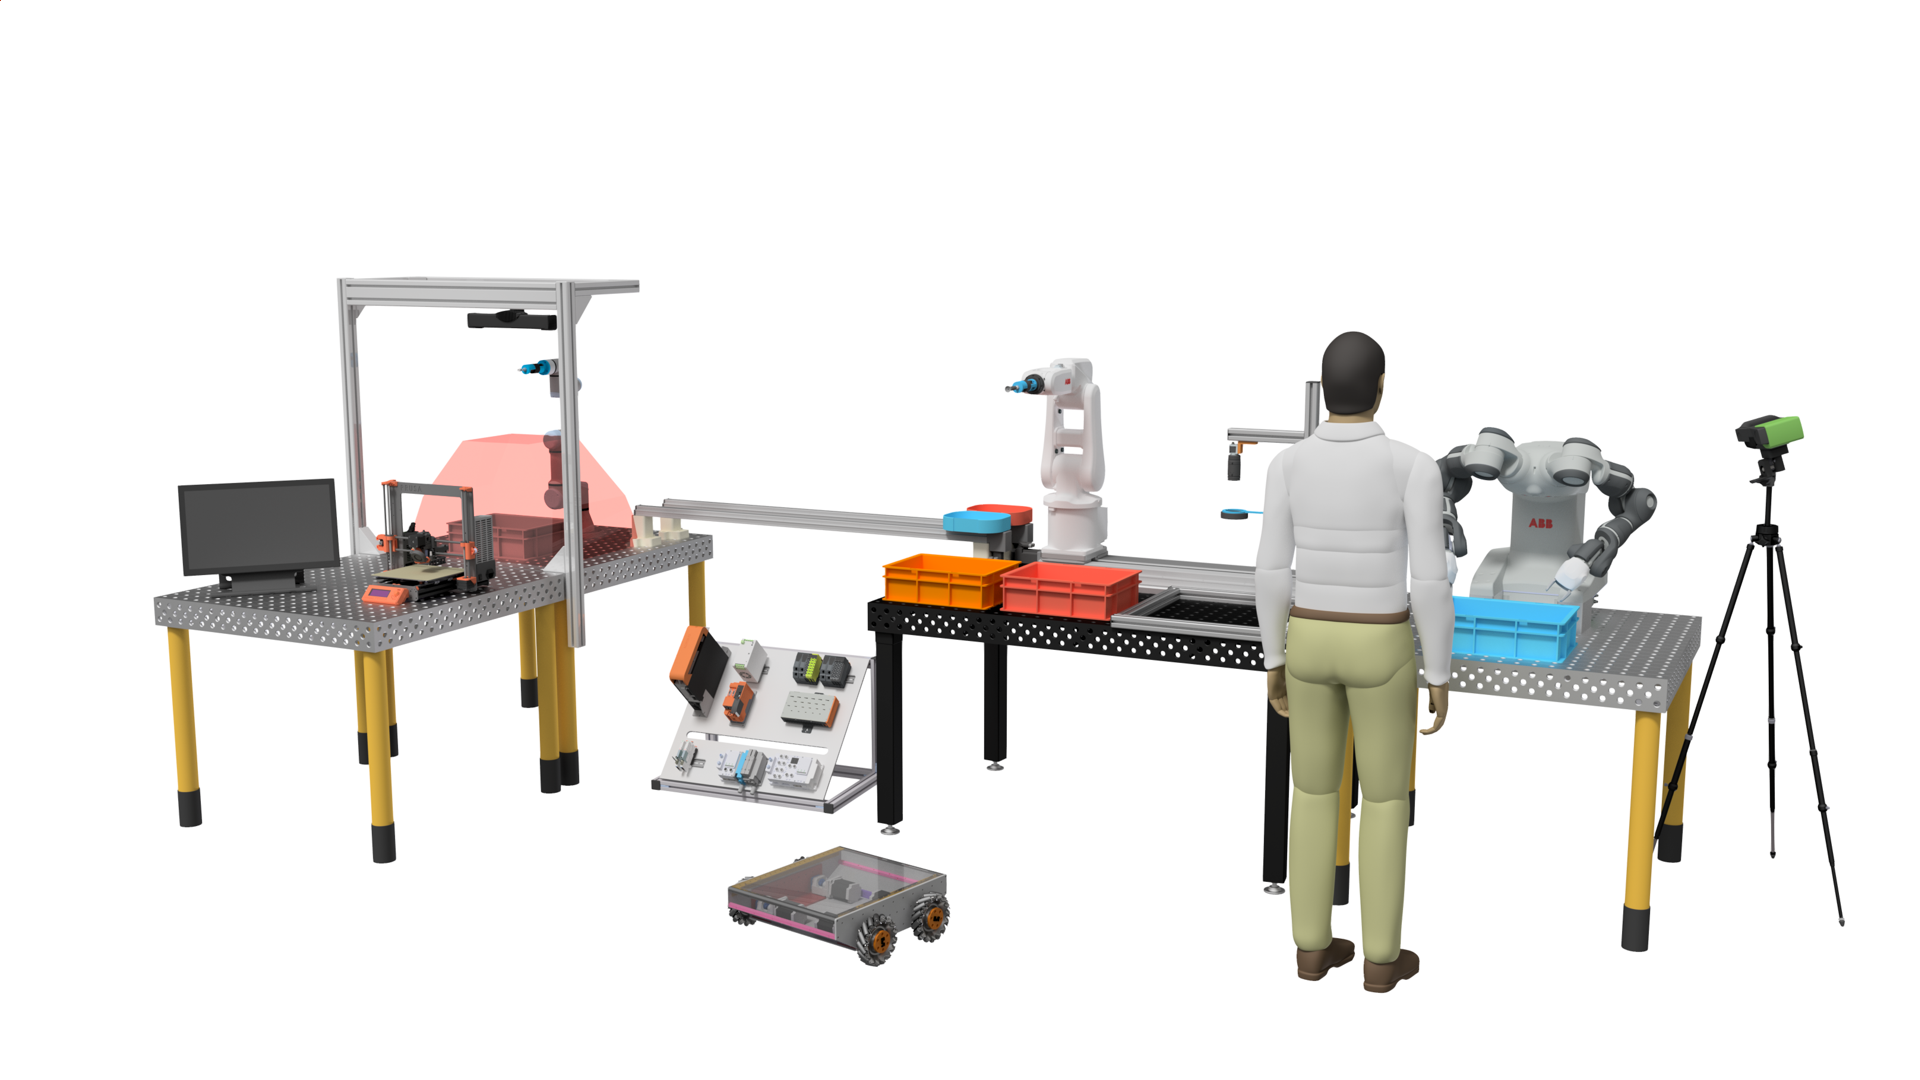
\includegraphics[scale=0.25]{image/i4c.png}
\caption{Please write your figure caption here}
\label{fig:1}
\end{center}
\end{figure}


%
% For tables use
%
\begin{table}[h] 
\begin{center}
\caption{Please write your table caption here} 
\label{tab:1}
\begin{tabular}{lll}
\hline\noalign{\smallskip}
Parameter & Symbol & Value\\
\noalign{\smallskip}
\hline\noalign{\smallskip}
Param no. 1 & $\delta$ & 0\\
Param no. 2 & $\pi$    & 3.14\\
\hline
\end{tabular}
\end{center}
\end{table}

\section{Conclusion}
\label{sec:2}
\blindtext

% References
%
\begingroup
\makeatletter
\renewcommand\section{\@startsection {section}{1}{\z@}%
                                   {-3.5ex \@plus -1ex \@minus -.2ex}%
                                   {4.5ex \@plus.2ex}%
                                   {\large\bfseries}}
\makeatother


\bibliography{references}{}
\bibliographystyle{acm}
\endgroup

\end{document}